\documentclass[11pt]{article}
\usepackage[UTF8]{ctex}
\usepackage[a4paper]{geometry}
\geometry{left=2.0cm,right=2.0cm,top=2.5cm,bottom=2.5cm}

\usepackage{caption}
\usepackage{paralist}
\usepackage{enumitem}
\setenumerate[1]{itemsep=0pt,partopsep=0pt,parsep=0pt,topsep=0pt}
\setitemize[1]{itemsep=0pt,partopsep=0pt,parsep=0pt,topsep=0pt}
\usepackage{comment}
\usepackage{booktabs}
\usepackage{graphicx}
\usepackage{float}
\usepackage{diagbox}
\usepackage{amsmath,amsfonts,graphicx,amssymb,bm,amsthm}
\usepackage{algorithm,algorithmicx}
% \usepackage[ruled, linesnumbered]{algorithm2e}
% \usepackage[linesnumbered]{algorithm2e}
\usepackage[noend]{algpseudocode}
\usepackage{fancyhdr}
\usepackage{tikz}
\usepackage{graphicx}
\usetikzlibrary{arrows,automata,positioning}
\usepackage{hyperref}
\usepackage{extarrows}
\usepackage{wrapfig}
% 这是一些字体选项
\usepackage{helvet}
% \usepackage{mathpazo}
\usepackage{fontspec}
% \setmainfont{Times New Roman}
% \setmainfont{Comic Sans MS} % 比较fancy的字体
% \setmainfont{Avenir}
% \setmainfont{Palatino}

\setlength{\headheight}{14pt}
\setlength{\parindent}{0 in}
\setlength{\parskip}{0.5 em}


\newtheorem{theorem}{Theorem}
\newtheorem{lemma}[theorem]{Lemma}
\newtheorem{proposition}[theorem]{Proposition}
\newtheorem{claim}[theorem]{Claim}
\newtheorem{corollary}[theorem]{Corollary}
\newtheorem{definition}[theorem]{Definition}
\newtheorem*{definition*}{Definition}

\newenvironment{problem}[2][Problem]{\begin{trivlist}
\item[\hskip \labelsep{\bfseries#1}\hskip\labelsep{\bfseries#2.}]}{\hfill$\blacktriangleleft$\end{trivlist}}
% 标题后强制换行
% \newenvironment{problem}[2][Problem]{\begin{trivlist}
%     \item[\hskip \labelsep{\bfseries#1}\hskip\labelsep{\bfseries#2.}]\mbox{}\newline}{\hfill$\blacktriangleleft$\end{trivlist}}
\newenvironment{answer}[1][Answer]{\begin{trivlist}
\item[\hskip \labelsep{\bfseries\itshape#1.}\hskip \labelsep]}{\hfill$\lhd$\end{trivlist}}

\DeclareMathOperator*{\minimize}{minimize}
\DeclareMathOperator*{\maximize}{maximize}
\newcommand\E{\mathbb{E}}
\newcommand\per{\mathrm{per}}
\renewcommand{\algorithmicrequire}{\textbf{Input:}}
\renewcommand{\algorithmicensure}{\textbf{Output:}}
\algrenewcommand{\algorithmiccomment}[1]{\hfill $//$ #1}
% chktex-file 44
% \renewcommand{\familydefault}{\sfdefault}

\RequirePackage{algorithm}

\makeatletter
\newenvironment{breakablealgorithm}
  {% \begin{breakablealgorithm}
    \begin{center}
      \refstepcounter{algorithm}% New algorithm
      \hrule height.8pt depth0pt \kern2pt% \@fs@pre for \@fs@ruled
      \parskip 0pt
      \renewcommand{\caption}[2][\relax]{% Make a new \caption
        {\raggedright\textbf{\fname@algorithm~\thealgorithm} ##2\par}%
        \ifx\relax##1\relax % #1 is \relax
          \addcontentsline{loa}{algorithm}{\protect\numberline{\thealgorithm}##2}%
        \else % #1 is not \relax
          \addcontentsline{loa}{algorithm}{\protect\numberline{\thealgorithm}##1}%
        \fi
        \kern2pt\hrule\kern2pt
     }
  }
  {% \end{breakablealgorithm}
     \kern2pt\hrule\relax% \@fs@post for \@fs@ruled
   \end{center}
  }
\makeatother

% set for automata
\tikzset{>=stealth',shorten >=1pt,auto,node distance=2cm, % Increase node distance to 4cm
                    thick,main node/.style={circle,draw,font=\sffamily\Large\bfseries}}


\title{Homework \#5}
\usetikzlibrary{positioning}

\begin{document}
\captionsetup[figure]{labelfont={bf},name={Fig.},labelsep=period}
\kaishu

\pagestyle{fancy}
\lhead{\CJKfamily{zhkai} Peking University}
\chead{}
\rhead{\CJKfamily{zhkai} Algorithm Design and Analysis (Honor Track)}

\begin{center}
    {\LARGE \bf Homework 6}\\
    {Name: 方嘉聪\ \  ID: 2200017849}            % Write down your name and ID here.
\end{center}

\begin{problem}{1. (Aggregate Analysis and Accounting Method)}
    Suppose we have a data structure where the cost $T(i)$ of the $i$-th operation is:
\begin{equation*}
    T(i)=
    \begin{cases}
    2i &\text{if }i \text{ is a power of }2, \\
    1 &\text{otherwise}.
    \end{cases}
\end{equation*}
What is the amortized cost of the operation? Use both the aggregate method and the accounting method to analyze the amortized running time.
\end{problem}
\begin{answer}
    操作的均摊代价为$O(1)$.
    \begin{enumerate}[label = (\alph*)]
        \item \textbf{Aggregate Method: } 对$\forall n$, 设操作的总代价为$S(n)$, 则有:
        \begin{align*}
            S(n) &= \sum_{i=0}^{\log \left\lfloor n \right\rfloor} 2^{i+1} + n - \log \left\lfloor n \right\rfloor - 1 \\
            &= 2^{\log \left\lfloor n \right\rfloor + 2} + n - \log \left\lfloor n \right\rfloor - 2 \\
            &= 4\left\lfloor n \right\rfloor  + n - \log \left\lfloor n \right\rfloor - 2 \\
            &\implies \frac{S(n)}{n} < 5
        \end{align*}
        故每个操作的均摊代价为$O(1)$.
        \item \textbf{Accounting Method: }设第$i$个操作的均摊代价为$T'(i)$. $\forall k \in \mathbb{N}$, 
        
        1. 对于$2^k < m < 2^{k+1}$, 令$T'(m) = 5$, 其中多出的$4$单位代价存储在第$2^{k+1}$的账上.

        2. 对于$m = 2^k$, 令$T'(m) = 0$, 此时加上之前存储的$4 \cdot 2^{k-1} = 2^{k+1}$恰好抵消了实际的代价.

        显然$\sum_{i=0}^{k} T(i) \le \sum_{i=0}^{k} T'(i)$, 故每个操作的均摊代价为$O(1)$.
    \end{enumerate}
\end{answer}

\begin{problem}{2. (Potential Method)}
  We want to design a data structure $S$ with \textbf{real numbers}, with the following two operations: 

  1) $\mathtt{insert}(S,x)$ inserts the object $x$ in $S$.
  
  2) $\mathtt{delete}(S)$ removes the $\left\lceil|S|/2\right\rceil$ largest elements of $S$. 
  
  Propose your implementation of the data structure and analyze the amortized costs of the two operations with potential method, such that the amortized runtime of $\mathtt{insert}(S,x)$ is $O(1)$, and that of $\mathtt{delete}(S)$ is 0.

  (\textit{Hint: Remember that you can find the median of a list in linear time.})
\end{problem}
\begin{answer}
我们用一个单链表来存储数据, 每个链表节点存储实数$x$, 并有势能函数$\Phi$.

1. $\mathtt{insert}(S, x)$操作: 将元素添加到链表的末尾, 代价为$\Theta(1)$.

2. $\mathtt{delete}(S)$操作: 首先找到链表的中位数(使用课上提到的确定性选择算法, 复杂度为$O(n)$), 然后遍历链表, 将大于中位数的元素删除, 代价为$\Theta(n)$.

设链表的长度为$n$, $\mathtt{delete}(S)$操作的时间复杂度的上界为$cn$(其中$c$为常数), 我们定义势能函数为
\[\Phi = 2cn\]
注意到初始状态$n = 0$, 势能函数$\Phi$是非负的. 那么, 两种操作的均摊代价为:
\begin{enumerate}
    \item  $\mathtt{insert}(S, x)$操作的均摊代价为$1 + \Phi(n) - \Phi(n-1) = 1 + 2c = \Theta(1)$.
    \item  $\mathtt{delete}(S)$操作的均摊代价为$cn + \Phi(\left\lceil n/2\right\rceil) - \Phi(n) = 0$.
\end{enumerate}
满足题设的条件.

注: 如果考虑元素可能相同, 那么在$\mathtt{delete}(S)$操作中可以先将不小于中位数的元素全部删除, 如果删除的元素个数大于$\left\lceil n/2\right\rceil$, 那么调用$\mathtt{insert}(S, x)$操作对应次数即可, 此时的时间复杂度还是$\Theta(n)$, 上述的分析仍成立.
\end{answer}

\begin{problem}{3. (LP Formulation)}
    Formulate the following problems as LPs:

    (a) minimize $||Ax-b||_1$ subject to $||x||_{\infty} \leqslant 1$.
    
    (b) minimize $||x||_1$ subject to $||Ax-b||_{\infty} \leqslant 1$.
    
    (c) minimize $||Ax-b||_1 + ||x||_{\infty}$.
    
    In each problem, $A\in \mathbb{R}^{m \times n}$ and $b \in \mathbb{R}^m$ are given, and $x\in \mathbb{R}^n$ is the optimization variable.
    
    ($||X||_1 = \sum_i|X_i|, ||X||_{\infty} = \max_i |X_i|$)
\end{problem}
\begin{answer}
    \begin{enumerate}[label = (\alph*)]
        \item 等价的线性规划问题为
        \begin{align*}
            \minimize \quad & \sum_{i=1}^{m} u_i \\
            \text{subject to} \quad & -u_i \leqslant a_i^T x - b_i \leqslant u_i, \quad i = 1, 2, \ldots, m, \\
            & -1 \leqslant x_j \leqslant 1, \quad j = 1, 2, \ldots, n.
        \end{align*}
        \item 等价的线性规划问题为
        \begin{align*}
            \minimize \quad & \sum_{i=1}^{n} u_i \\
            \text{subject to} \quad & - u_i \leqslant x_i \leqslant u_i, \quad i = 1, 2, \ldots, n, \\
            & -1 \leqslant a_i^T x - b_i \leqslant 1, \quad i = 1, 2, \ldots, m.
        \end{align*}
        \item 等价的线性规划问题为
        \begin{align*}
            \minimize \quad & \sum_{i=1}^{m} u_i + t \\
            \text{subject to} \quad & -u_i \leqslant a_i^T x - b_i \leqslant u_i, \quad i = 1, 2, \ldots, m, \\
            & -t \leqslant x_j \leqslant t, \quad j = 1, 2, \ldots, n.
        \end{align*}
    \end{enumerate}
    以上$A,b$为给定的, $u_i, t$为引入的辅助变量, $x \in \mathbb{R}^n$为优化变量. 

    注意到上述形式不是标准型但是可以通过课上提及的松弛技巧转化为标准型的线性规划问题, 这里为了简洁不再展开书写.
\end{answer}

\begin{problem}{4. (Construct a Hyperplane)}
    Describe a method for constructing a hyperplane that separates two given polyhedra:
    \begin{equation*}
    \mathcal{P}_1 = \{x\in \mathbb{R}^n | Ax \leqslant b\}, \mathcal{P}_2 = \{x\in \mathbb{R}^n | Cx \leqslant d\}.
    \end{equation*}
    Your method must return a vector $a\in \mathbb{R}^n$ and a scalar $\gamma$ such that
    \begin{equation*}
        a^T x > \gamma, \forall x\in \mathcal{P}_1;\ a^T x < \gamma, \forall x\in \mathcal{P}_2.
    \end{equation*}
    You can assume that $\mathcal{P}_1$ and $\mathcal{P}_2$ do not intersect. If you know several methods, you should give the most efficient one.
    
    \begin{figure}[H] 
        \centering
        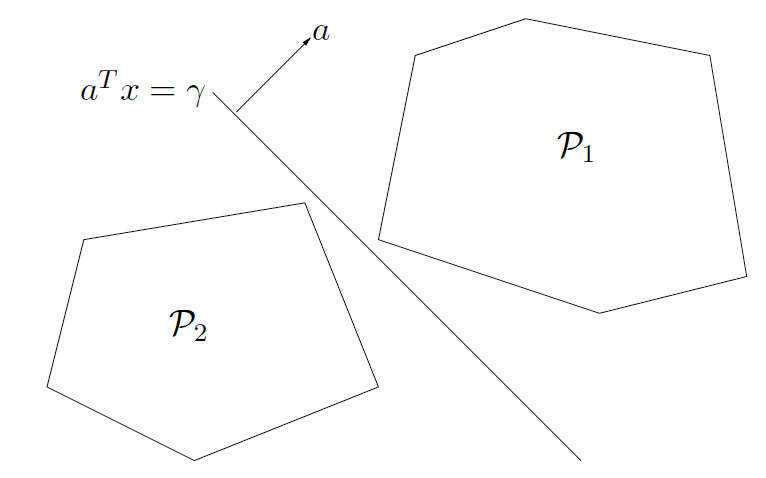
\includegraphics[width=0.4\textwidth]{figs/plane.png}
    \end{figure}
\end{problem}
\begin{answer}
    上述问题等价于寻找$a, \gamma$满足
    \begin{align*}
        \sup_{x \in \mathcal{P}_2} a^T x < \gamma < \inf_{x \in \mathcal{P}_1} a^T x.
    \end{align*}
    下面将这一问题转化为线性规划的形式(这样就是可解的), 设:
    \begin{align*}
        p_1^*(a) = \inf \{a^T x \mid A x \leqslant b\}, \quad p_2^*(a) = \sup \{a^T x \mid C x \leqslant d\}.
    \end{align*}
    那么为了找到满足条件的$a$, 相当于求解下面这个问题:
    \begin{align}
        \maximize \quad & p_1^*(a) - p_2^*(a) \label{4.1} \\ 
        \text{subject to} \quad & \left\|x\right\|_1 \leqslant 1.  \label{4.2}
    \end{align} 
    这里取约束(\ref{4.2})是由于$p_1^*(a) - p_2^*(a)$是齐次的, 如果不对其增加$a$的范数约束那么上述的问题是不可解的(\emph{unbounded}). 
    
    如果上述问题有解, 那么最优解$a^*$就是我们要找的$a$, 再令$\gamma = (p_1^*(a^*) + p_2^*(a^*))/2$即可.注意到
    \begin{align*}
        p_1^*(a) &= \inf\{a^T x \mid Ax \leqslant b\} = \sup\{-b^T z_1 \mid A^T z_1 + a = 0, z_1 \geqslant 0\} \\
        -p_2^*(a) &= \inf\{-a^T x \mid Cx \leqslant d\} = \sup\{-d^T z_2 \mid C^T z_2 - a = 0, z_2 \geqslant 0\} 
    \end{align*}
    上面的等式用到了线性规划的对偶形式. 那么问题(\ref{4.1})-(\ref{4.2})可以转化为下面的线性规划问题:
    \begin{align*}
        \maximize \quad & -b^T z_1 - d^T z_2 \\
        \text{subject to} \quad & A^T z_1 + a = 0, \quad z_1 \geqslant 0, \\
        & C^T z_2 - a = 0, \quad z_2 \geqslant 0, \\
        & \left\|a\right\|_1 \leqslant 1. 
    \end{align*}
    其中$a, z_1, z_2$为变量, $\left\|a\right\|_1 \leqslant 1$也可以写成$-1 \leqslant a_i \leqslant 1, i = 1, 2, \ldots, n$. 故只需要求解上述的线性规划问题(总共有$3n$个参数)即可找到满足条件的$a, \gamma$. 
\end{answer}


\end{document}